\section{Übung 2 - Fremdkapital}

\subsection{Kennzahlen Working Capital Management}
\begin{itemize}
	\item $\diameter$Lagerhaltungsdauer (DIO) $=\cfrac{\diameter\text{Lagerbestand}\cdot 360\text{ Tage}}{\text{Umsatzkosten}}=\cfrac{360\text{ Tage}}{\text{Lagerumschlagshäufigkeit}}$
	\item $\diameter$Inkassoperiode (DSO) $=\cfrac{\diameter\text{Forderungen aus L\&L}\cdot 360\text{ Tage}}{\text{Umsatz auf Ziel}}=\cfrac{360\text{ Tage}}{\text{Forderungsumschlagshäufigkeit}}$
	\item 
	$
		\begin{aligned}[t]
			\diameter\text{Kreditorenlaufzeit (DPO)} & = \cfrac{\diameter\text{Verbindlichkeiten aus L\&L}\cdot 360\text{ Tage}}{\text{Umsatzkosten}} \\
			& = \cfrac{360\text{ Tage}}{\text{Verbindlichkeitenumschlagshäufigkeit}}
		\end{aligned}$
	\item Operating Cycle (OC) $=\diameter\text{Lagerhaltungsdauer}+\diameter\text{Inkassoperiode}$
	\item Cash Conversion Cycle (CCC) $= \text{OC}-\diameter\text{Kreditorenlaufzeit}$
\end{itemize}

\subsection{Externer Finanzierungsbedarf}
\begin{itemize}
	\item $\text{Brutto-Finanzierungsbedarf}=\Delta\text{Liquide Mittel}+\Delta\text{NWC}+\text{Investitionen in Anlagevermögen}$
	\item $\text{Innenfinanzierung}=\text{Einbehaltener Gewinn}+\text{Abschreibungen}(+\text{Non-Cash Expenses})$
	\item $\text{Externer Finanzierungsbedarf}=\text{Brutto-Finanzierungsbedarf}-\text{Innenfinanzierung}$
\end{itemize}

\subsection{Fremdkapital: Unternehmensanleihen und Fremdkapitalkosten}
\textbf{Ausgestaltungsmerkmale von Anleihen}:
\begin{itemize}
	\item Höhe des Emissionsvolumens
	\item Kupon-Zinssatz
	\item Fälligkeit, Rückzahlungskurs
	\item Covenants: Nicht standardisierte, individuell vereinbarte Verpflichtungen für den Emittenten $\rightarrow$ Reduktion des Kreditrisikos der Kreditgeber
	\item Kündigungsrechte
\end{itemize}
\bigskip
\textbf{Anleihebewertung}:
\begin{itemize}
	\item Bewertung einer \textbf{Kuponanleihe}: $$P=\sum\limits_{t=1}^T \cfrac{\text{CPN}}{(1+\text{YTM})^t}+\cfrac{\text{FV}}{(1+\text{YTM})^T}\qquad$$
	mit CPN: Höhe des Kupons, YTM (Yield-to-Maturity): effektiver Zinssatz, FV (Face Value): Rückzahlungsbetrag (Nennwert + Kupon)
	\begin{center}
		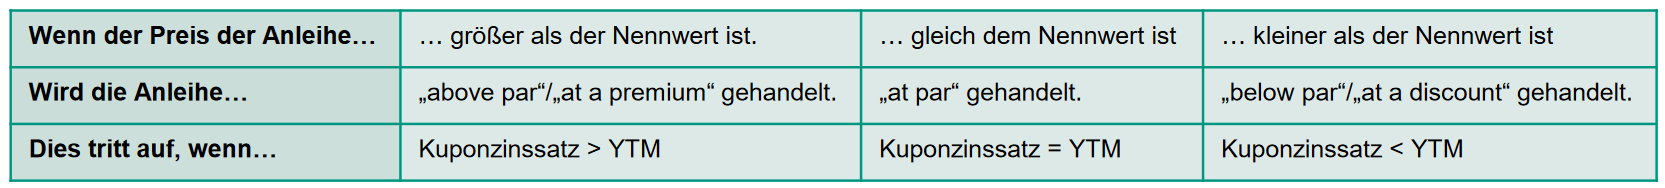
\includegraphics[width=\textwidth]{images/e5.png}
	\end{center}
	\item Bewertung einer \textbf{Nullkuponanleihe}: $P=\cfrac{\text{FV}}{(1+\text{YTM})^T}$
	\item Bewertung einer \textbf{ewigen Anleihe}: $P=\cfrac{\text{CPN}}{\text{YTM}}$
\end{itemize}

\textbf{Stückzinsen}: 
\begin{itemize}
	\item \textbf{Clean Price}: Quotierter Preis der Anleihe
	\item \textbf{Dirty Price}: Tatsächlich zu zahlender Preis bei Kauf der Anleihe $\rightarrow$ Höher als Clean Price wegen Stückzinsen
	\item $\text{Stückzinsen}=\text{Kuponbetrag}\cdot\cfrac{\text{Tage seit letzter Kuponzahlung}}{\text{Tage in aktueller Kuponperiode}}$
	\item $\text{Dirty Price}=\text{Clean Price}+\text{Stückzinsen}$
\end{itemize}

\textbf{Kreditrisiko / Ausfallrisiko}:
\begin{itemize}
	\item \textbf{Investment Grade}: BBB- und besser
	\item \textbf{Speculative Grade (High Yield)}: BB+ und schlechter
	\item \textbf{Credit Spread}: Risikoprämie einer riskanten Anleihe gegenüber einer vergleichbaren, risikolosen Anleihe
	\item \textbf{Duration}: Sensitivität einer Anleihe gegenüber Änderungen im Zinsniveau
\end{itemize}


